\documentclass[12pt,twocolumn]{IEEEtran}
\usepackage{amsfonts}
\usepackage{amsmath}
\usepackage{amssymb}
\usepackage[latin1]{inputenc}                                 
\usepackage{color}                                            
\usepackage{array}                                            
\usepackage{longtable}                                        
\usepackage{calc}                                             
\usepackage{multirow}                                         
\usepackage{hhline}                                           
\usepackage{ifthen}
\usepackage{enumitem}
\usepackage{graphicx}
\def\inputGnumericTable{}
\newcommand{\question}{\noindent \textbf{Question: }}
\newcommand{\solution}{\noindent \textbf{Solution: }}


\title{Assignment 3}
\author{Suraj kumar \\ \normalsize AI21BTECH11029\\ \Large CBSE 9th Statistics }
\begin{document}
\maketitle
\question  (Exercise 14.3 Q4) $\Rightarrow$ The length of 40 leaves of a plant are measured correct to one milimetre,and the obtained data is represented in the following table:
\begin{table}[ht!]
	\begin{center}
		
    \begin{tabular}{|c|c|}
        \hline
        Length(in mm) & Number of leaves \\ \hline
        118-126       & 3                \\ \hline
        127-135       & 5                \\ \hline
        136-144       & 9                \\ \hline
        145-153       & 12               \\ \hline
        154-162       & 5                \\ \hline
        163-171       & 4                \\ \hline
        172-180       & 2                \\ \hline
    \end{tabular}

		\vspace*{3pt}
		\caption{}
		\label{table:table1}
	\end{center}
\end{table}
\begin{enumerate}[label=(\roman*)]
	\item Draw a histogram to represent the given data.
	\item Is there any other suitable graphical representation for the same data?
	\item Is it correct to conclude that the maximum number of leaves are $153$ mm long ? why?
\end{enumerate}
\solution
\begin{enumerate}[label=(\roman*)]
	\item The data given in the question is represented in discountinuous class interval. So, we have to make it in continuous class interval.the difference is $1$,so taking half of $1$ ,we subtract $1/2=0.5$ from lower limit and add $0.5$ to the upper limit.Then the table becomes:
	      \begin{table}[ht!]
		      \begin{center}
			      \centering
\begin{tabular}{|c|c|}
\hline
    Length (in mm) & Number of leaves \\ \hline
    117.5-126.5 & 3 \\ \hline
    126.5-135.5 & 5 \\ \hline
    135.5-144.5 & 9 \\ \hline
    144.5-153.5 & 12 \\ \hline
    153.5-162.5 & 5 \\ \hline
    162.5-171.5 & 4 \\ \hline
    171.5-180.5 & 2 \\ \hline
\end{tabular}
			      \vspace*{3pt}
			      \caption{}
			      \label{table:table2}
		      \end{center}
	      \end{table}
	      \begin{figure}[ht!]
		      \begin{center}
			      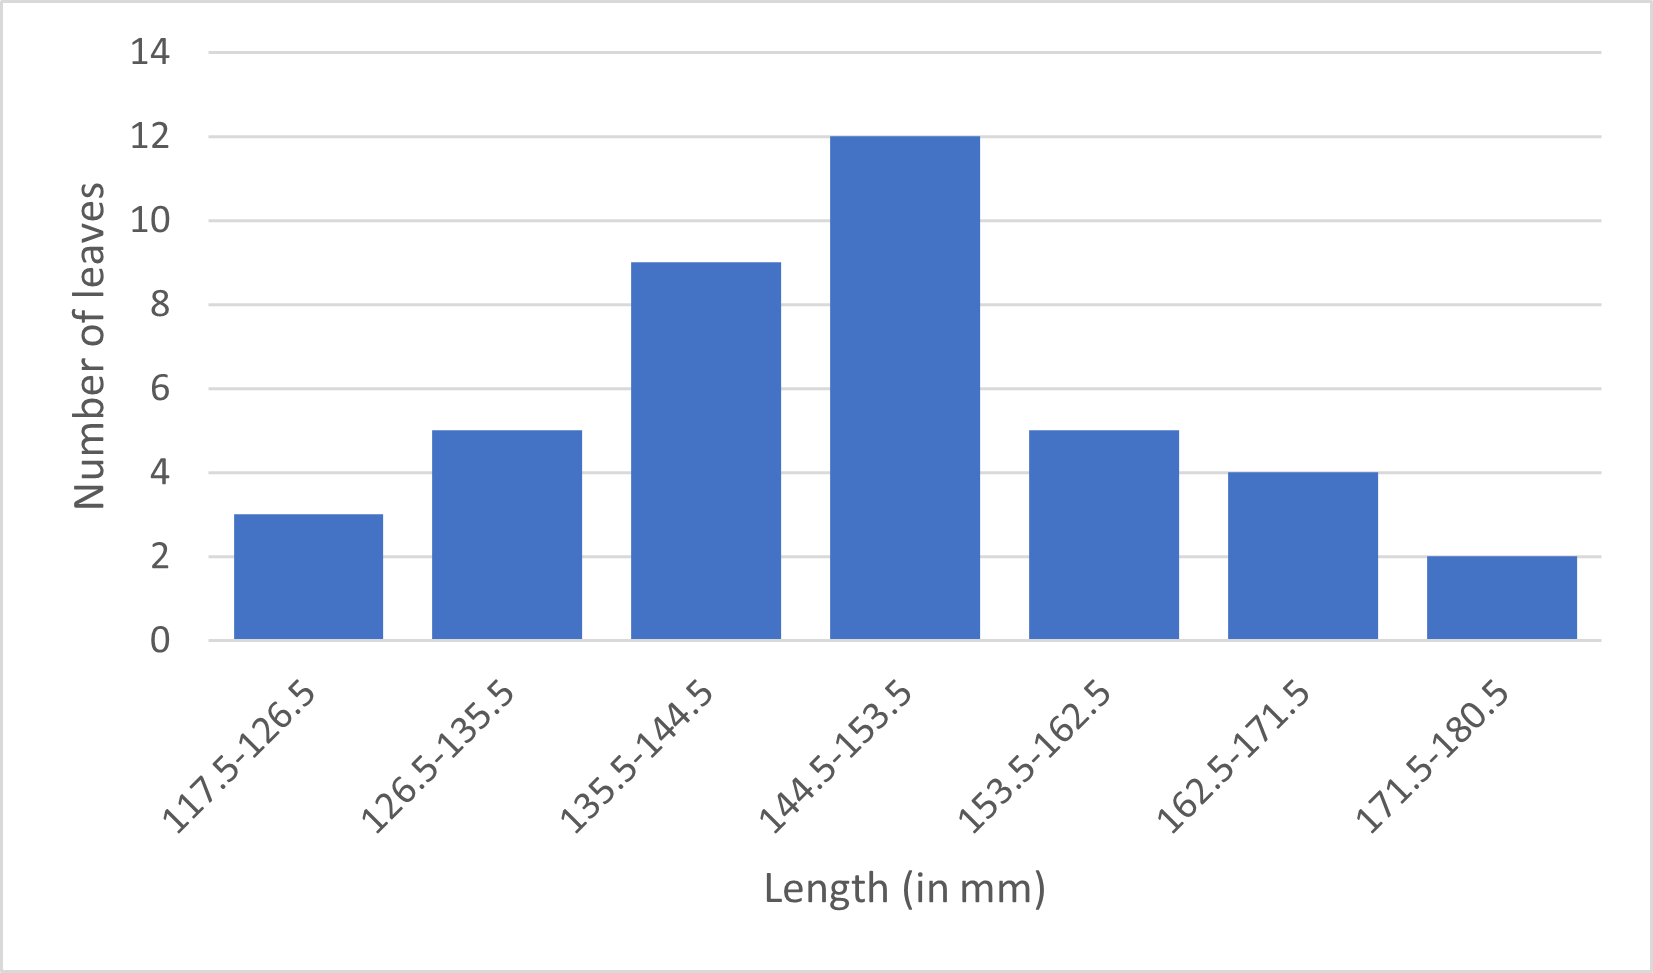
\includegraphics[width=\columnwidth]{fig/Picture1.png}
			      \caption{}
			      \label{fig:fig1}
		      \end{center}

	      \end{figure}
		  \pagebreak
	\item Yes ,the data given in the question can also be represented by frequency polygon.
	\begin{figure}[ht!]
		\begin{center}
			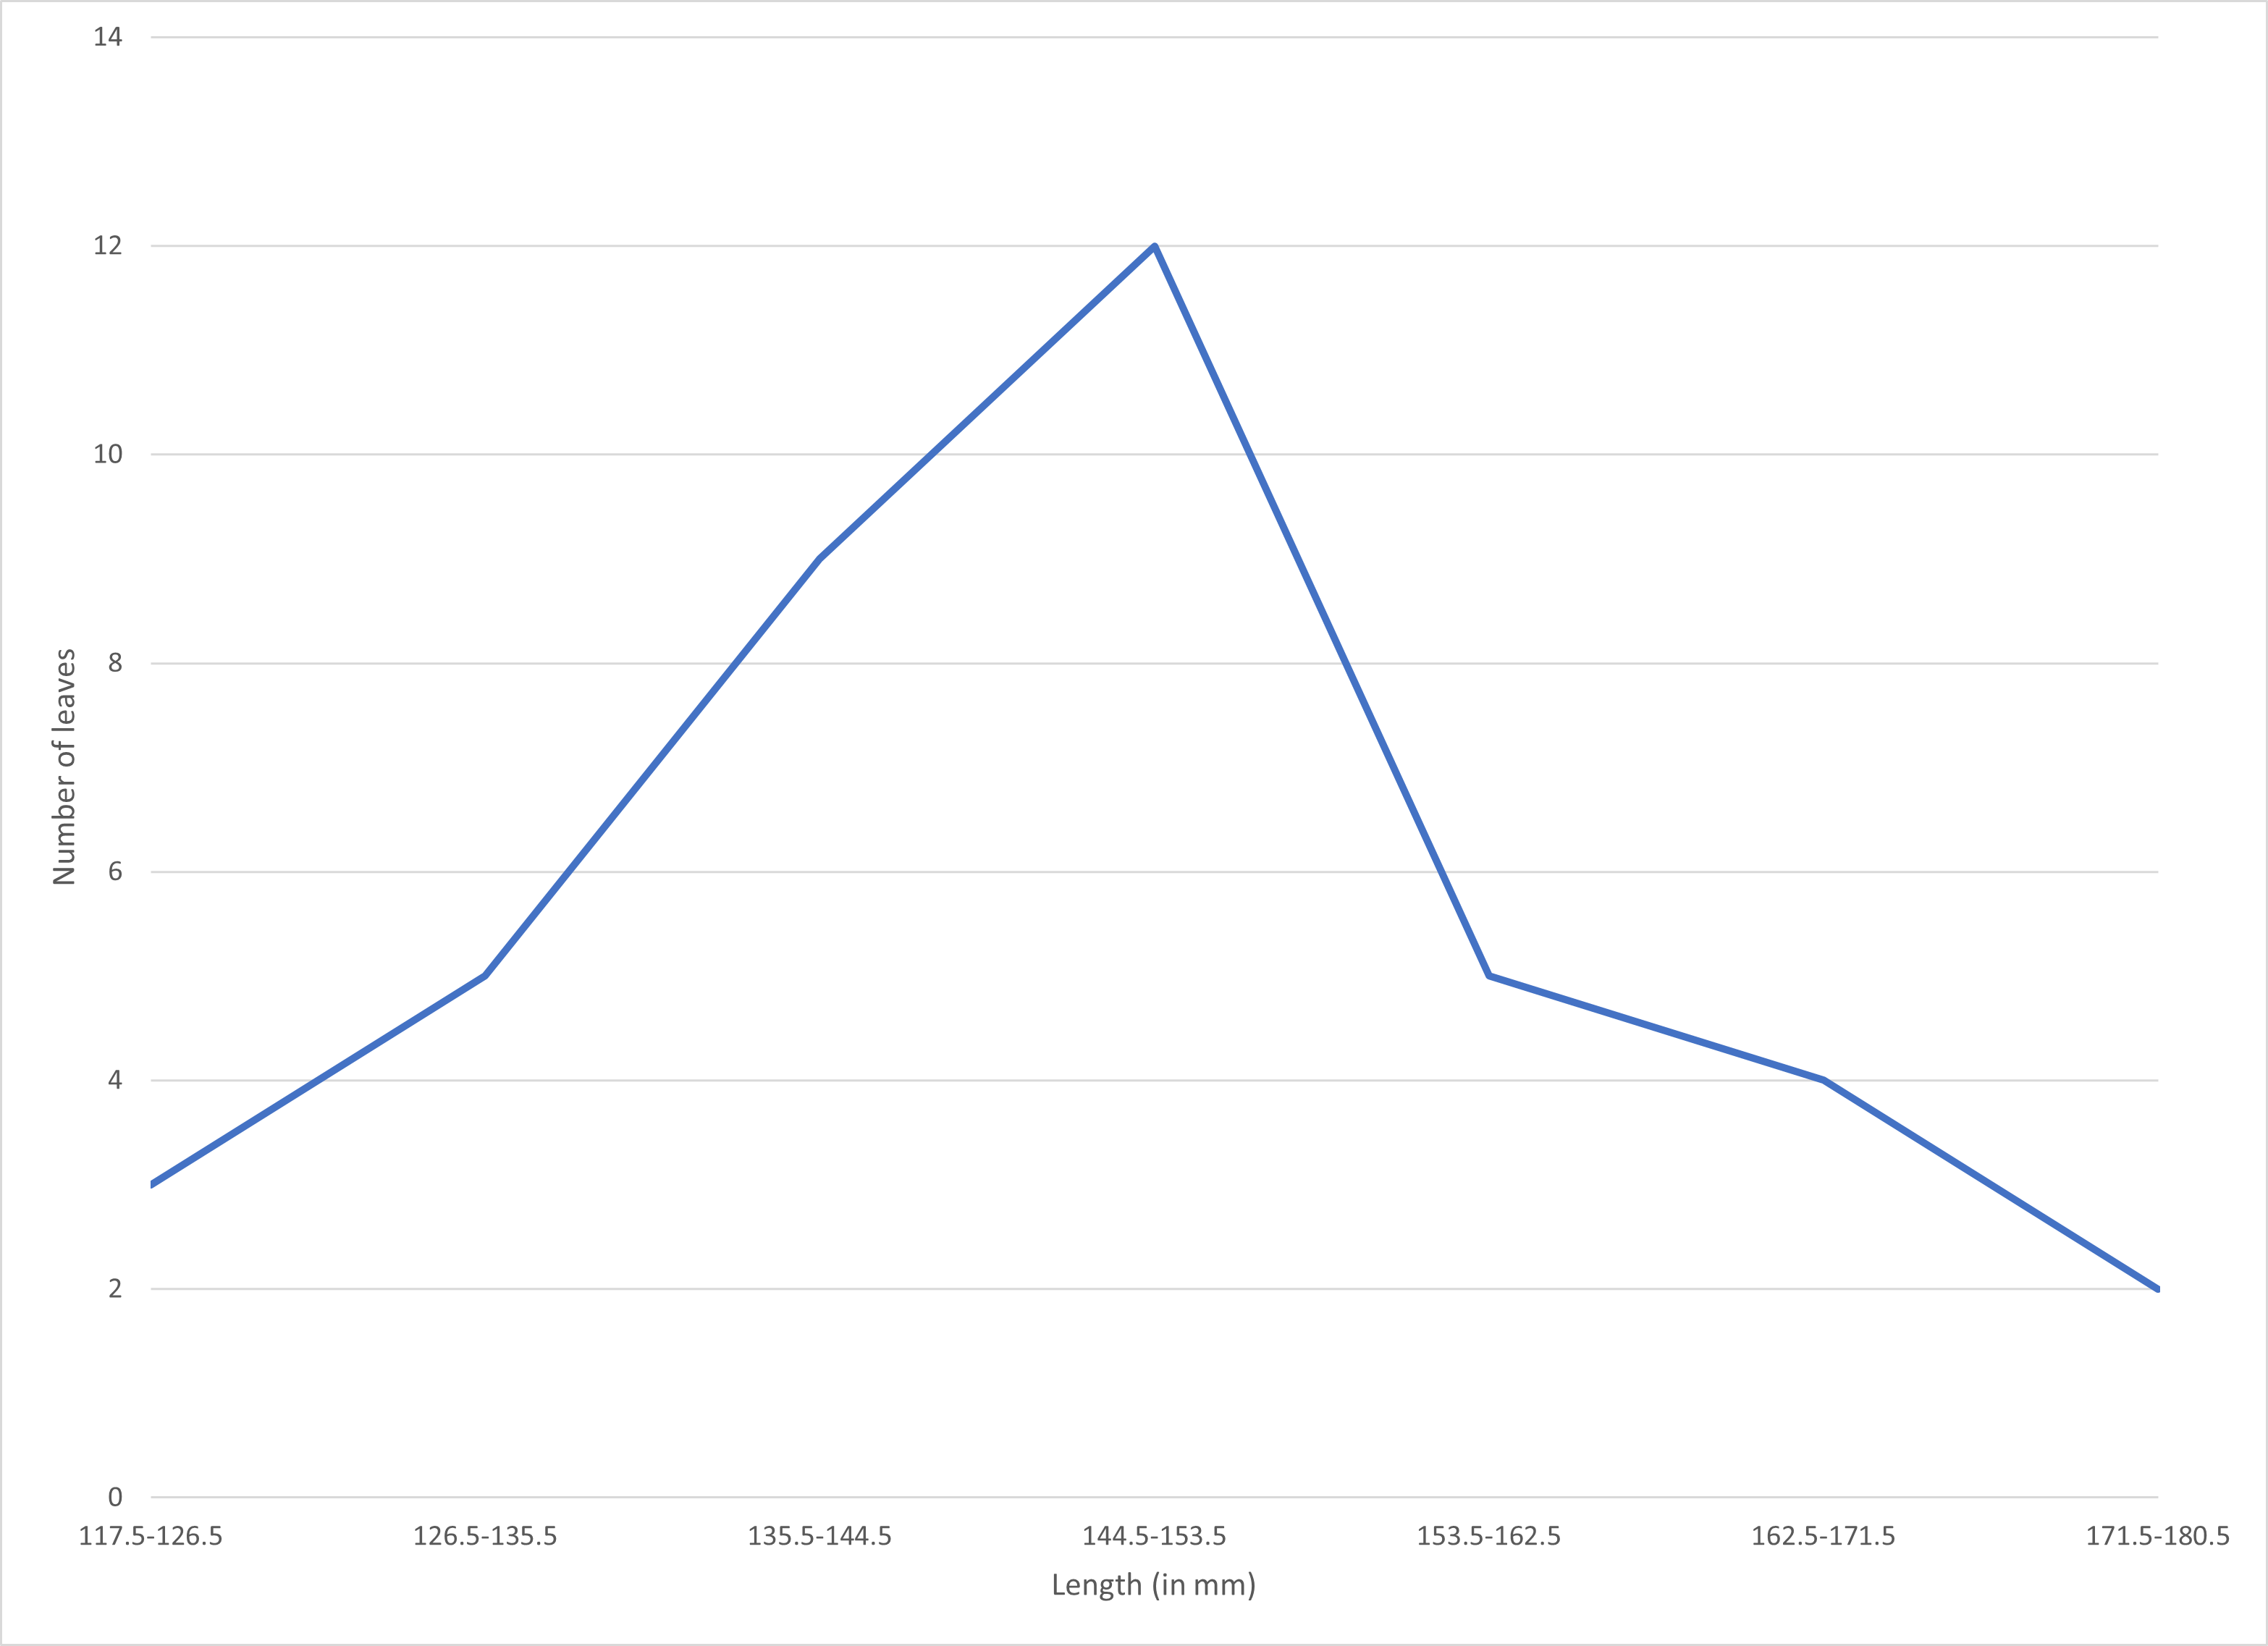
\includegraphics[width=\columnwidth]{fig/Picture2.png}
			\caption{}
			\label{fig:fig2}
		\end{center}

	\end{figure}
	\item No,we cannot conclude that the maximum number of leaves are $153$mm long because the maximum number of leaves are lying in-between the length of $144.5-153.5$


\end{enumerate}
\end{document}